\documentclass[tikz,border=4pt]{standalone}
\usepackage{tikz}
\usetikzlibrary{arrows.meta,calc}
\begin{document}
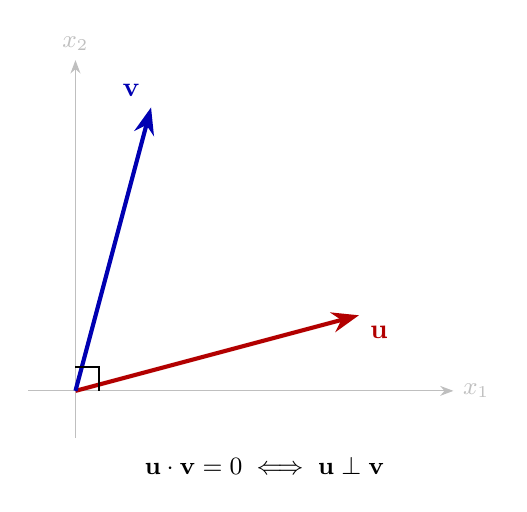
\begin{tikzpicture}[>=Stealth, scale=1.2]
    % Axes
    \draw[->,gray!50] (-0.5,0) -- (4,0) node[right,font=\small] {$x_1$};
    \draw[->,gray!50] (0,-0.5) -- (0,3.5) node[above,font=\small] {$x_2$};

    % Vector u
    \draw[->,red!70!black,line width=1.5pt] (0,0) -- (3,0.8)
        node[below right,font=\bfseries] {$\mathbf{u}$};

    % Vector v (perpendicular)
    \draw[->,blue!70!black,line width=1.5pt] (0,0) -- (0.8,3)
        node[above left,font=\bfseries] {$\mathbf{v}$};

    % Right angle mark
    \draw[thick] (0.25,0) -- (0.25,0.25) -- (0,0.25);

    % Formula
    \node[font=\small,anchor=north] at (2,-0.6)
        {$\mathbf{u}\cdot\mathbf{v} = 0 \;\Longleftrightarrow\; \mathbf{u} \perp \mathbf{v}$};
\end{tikzpicture}
\end{document}
